% Options for packages loaded elsewhere
\PassOptionsToPackage{unicode}{hyperref}
\PassOptionsToPackage{hyphens}{url}
%
\documentclass[
  12pt,
]{article}
\usepackage{lmodern}
\usepackage{amssymb,amsmath}
\usepackage{ifxetex,ifluatex}
\ifnum 0\ifxetex 1\fi\ifluatex 1\fi=0 % if pdftex
  \usepackage[T1]{fontenc}
  \usepackage[utf8]{inputenc}
  \usepackage{textcomp} % provide euro and other symbols
\else % if luatex or xetex
  \usepackage{unicode-math}
  \defaultfontfeatures{Scale=MatchLowercase}
  \defaultfontfeatures[\rmfamily]{Ligatures=TeX,Scale=1}
\fi
% Use upquote if available, for straight quotes in verbatim environments
\IfFileExists{upquote.sty}{\usepackage{upquote}}{}
\IfFileExists{microtype.sty}{% use microtype if available
  \usepackage[]{microtype}
  \UseMicrotypeSet[protrusion]{basicmath} % disable protrusion for tt fonts
}{}
\makeatletter
\@ifundefined{KOMAClassName}{% if non-KOMA class
  \IfFileExists{parskip.sty}{%
    \usepackage{parskip}
  }{% else
    \setlength{\parindent}{0pt}
    \setlength{\parskip}{6pt plus 2pt minus 1pt}}
}{% if KOMA class
  \KOMAoptions{parskip=half}}
\makeatother
\usepackage{xcolor}
\IfFileExists{xurl.sty}{\usepackage{xurl}}{} % add URL line breaks if available
\IfFileExists{bookmark.sty}{\usepackage{bookmark}}{\usepackage{hyperref}}
\hypersetup{
  pdftitle={Turnout and Amendment 4: Mobilizing Eligible Voters Close to the Disenfranchised},
  pdfauthor={Kevin Morris},
  hidelinks,
  pdfcreator={LaTeX via pandoc}}
\urlstyle{same} % disable monospaced font for URLs
\usepackage[margin=1in]{geometry}
\usepackage{longtable,booktabs}
% Correct order of tables after \paragraph or \subparagraph
\usepackage{etoolbox}
\makeatletter
\patchcmd\longtable{\par}{\if@noskipsec\mbox{}\fi\par}{}{}
\makeatother
% Allow footnotes in longtable head/foot
\IfFileExists{footnotehyper.sty}{\usepackage{footnotehyper}}{\usepackage{footnote}}
\makesavenoteenv{longtable}
\usepackage{graphicx}
\makeatletter
\def\maxwidth{\ifdim\Gin@nat@width>\linewidth\linewidth\else\Gin@nat@width\fi}
\def\maxheight{\ifdim\Gin@nat@height>\textheight\textheight\else\Gin@nat@height\fi}
\makeatother
% Scale images if necessary, so that they will not overflow the page
% margins by default, and it is still possible to overwrite the defaults
% using explicit options in \includegraphics[width, height, ...]{}
\setkeys{Gin}{width=\maxwidth,height=\maxheight,keepaspectratio}
% Set default figure placement to htbp
\makeatletter
\def\fps@figure{htbp}
\makeatother
\setlength{\emergencystretch}{3em} % prevent overfull lines
\providecommand{\tightlist}{%
  \setlength{\itemsep}{0pt}\setlength{\parskip}{0pt}}
\setcounter{secnumdepth}{5}
\usepackage{rotating}
\usepackage{setspace}
\usepackage{booktabs}
\usepackage{longtable}
\usepackage{array}
\usepackage{multirow}
\usepackage{wrapfig}
\usepackage{float}
\usepackage{colortbl}
\usepackage{pdflscape}
\usepackage{tabu}
\usepackage{threeparttable}
\usepackage{threeparttablex}
\usepackage[normalem]{ulem}
\usepackage{makecell}
\usepackage{xcolor}
\newlength{\cslhangindent}
\setlength{\cslhangindent}{1.5em}
\newenvironment{cslreferences}%
  {\setlength{\parindent}{0pt}%
  \everypar{\setlength{\hangindent}{\cslhangindent}}\ignorespaces}%
  {\par}

\title{Turnout and Amendment 4: Mobilizing Eligible Voters Close to the Disenfranchised\thanks{The author thanks Myrna Pérez, Patrick Berry, and Peter Miller for their comments on this project. All errors are my responsibility.}}
\author{Kevin Morris\footnote{Researcher, Brennan Center for Justice at NYU School of Law, 120 Broadway Ste 1750, New York, NY 10271 (\href{mailto:kevin.morris@nyu.edu}{\nolinkurl{kevin.morris@nyu.edu}})}}
\date{August 03, 2020}

\begin{document}
\maketitle
\begin{abstract}
Recent scholarship has established a link between felony disenfranchisement and lower turnout, particularly in Black communities. Little work, however, has been done to interrogate how this depressive effect might be counteracted. In 2018, Amendment 4 was on the ballot in Florida, and promised to re-enfranchise most of the disenfranchised population. The presence of this ballot initiative offers a unique opportunity to investigate whether ballot initiatives of special interest to these impacted communities might recoup their depressed turnout. Using individual-level release records from the Florida Department of Corrections I test whether the ballot initiative mobilized neighborhoods and individuals in close proximity to formerly incarcerated individuals. Using multiple identification strategies, I find no evidence that Amendment 4 increased the turnout of these eligible voters, indicating that (re)incorporating their voices into American democracy might be even harder than formerly recognized.
\end{abstract}

\pagenumbering{gobble}
\pagebreak

\pagenumbering{arabic}
\doublespacing

\hypertarget{introduction}{%
\section*{Introduction}\label{introduction}}
\addcontentsline{toc}{section}{Introduction}

On November 6\textsuperscript{th}, 2018, Floridians voted to amend their state constitution to re-enfranchise individuals with felony convictions in their past (Taylor \protect\hyperlink{ref-Taylor2018}{2018}). The move was hailed as transformational for Floridian --- and American --- democracy (Morris \protect\hyperlink{ref-Morris2018}{2018}); Uggen, Larson, and Shannon (\protect\hyperlink{ref-sentencing_2016}{2016}) had estimated a few years earlier that some 1.5 million Floridians were disenfranchised and had finished serving their sentences, making the amendment the largest expansion of the franchise in the United States since the Twenty-sixth Amendment lowered the voting age to 18. The racial implications for the constitutional amendment were also clear: according to the same Uggen, Larson, and Shannon (\protect\hyperlink{ref-sentencing_2016}{2016}) report, more than 1 out of every 5 Black Floridians was prohibited from democratic participation because of the state's disenfranchisement policies. Importantly, the amendment received broad support. Although it needed just 60 percent of the vote to pass, precinct-level data from the Florida Division of Elections shows that 64.5 percent of voters supported the ballot initiative. Conversely, the winning candidates for Governor and United States Senate won just 49.5 and 49.9 percent of the vote, respectively, implying that the constitutional amendment enjoyed substantial bipartisan support.

Felony disenfranchisement is not unique to Florida's electoral system: in all but two states in the United States, individuals convicted of felony offenses lose their right to vote for at least some period of time (Justice \protect\hyperlink{ref-bcj_laws}{2019}). According to the Brennan Center for Justice, felony convictions result in lifetime prohibitions from voting for some citizens in 11 states based on the severity of the crime.\footnote{Iowa stands alone in disenfranchising all individuals ever convicted of felony offenses (``Voting Rights Restoration Efforts in Iowa'' \protect\hyperlink{ref-bcj_iowa}{2020}).} Nevertheless, the shift in Florida from permanent disenfranchisement for all individuals convicted of felony offenses to restoring voting rights to most individuals\footnote{Individuals convicted of felony sexual assault or murder remain permanently disenfranchised.} upon the completion of their sentence moved the needle significantly: post-sentence Floridians accounted for roughly 24 percent of all disenfranchised Americans as of 2016 (Uggen, Larson, and Shannon \protect\hyperlink{ref-sentencing_2016}{2016}).

Amendment 4 was somewhat unique in how it restored voting rights. Usually, the question of voting rights restoration is not put directly to the voters. In New York State in 2018 (Wang \protect\hyperlink{ref-Wang2018}{2018}) and Kentucky in 2019 (Wines \protect\hyperlink{ref-Wines2019}{2019}), for instance, governors signed executive orders restoring voting rights to some disenfranchised individuals. In other states such as Louisiana (Crisp \protect\hyperlink{ref-Crisp2019}{2019}) and Colorado (Baumann \protect\hyperlink{ref-Baumann2019}{2019}) state lawmakers have passed bills restoring voting rights to formerly incarcerated individuals. Florida, however, did put the question directly to voters. In the Sunshine State, the general electorate had the opportunity to democratically decide whether they wanted to restore voting rights to their formerly incarcerated or probationed neighbors.

This paper explores whether the direct democratic approach of Amendment 4 increased participation among individuals who live in close proximity to the (formerly) disenfranchised. There is some literature that establishes that proximal contact with the criminal justice system reduces eligible Americans' propensity to vote (e.g.~Bowers and Preuhs \protect\hyperlink{ref-Bowers2009}{2009}; Burch \protect\hyperlink{ref-Burch2013}{2013}; King and Erickson \protect\hyperlink{ref-King2016}{2016}; Morris \protect\hyperlink{ref-Morris2020}{2020}). Little work, however, has been done exploring whether the opportunity to re-enfranchise family and community members can bring back these lost votes. The case of Amendment 4 in Florida offers a unique opportunity to investigate whether these eligible individuals can be reincorporated into our democratic processes. This project asks whether turnout in neighborhoods and households impacted by felony disenfranchisement were more likely to vote in 2018 than less-impacted groups and relative to their own participation history.

\hypertarget{theory-and-literature}{%
\section*{Theory and Literature}\label{theory-and-literature}}
\addcontentsline{toc}{section}{Theory and Literature}

It well established that direct contact with the criminal justice system reduces voter turnout (see, for instance, Weaver and Lerman \protect\hyperlink{ref-Weaver2010}{2010}; Burch \protect\hyperlink{ref-Burch2011}{2011}; White \protect\hyperlink{ref-White2019}{2019}\protect\hyperlink{ref-White2019}{b}). The evidence that ``proximal contact'' (Walker \protect\hyperlink{ref-Walker2014}{2014}) with the criminal justice system via family members and neighbors reduces turnout, however, is somewhat mixed. Though most research conducted in this area concludes that there are likely some negative ``spillover'' effects on turnout, others disagree. Some research finds that turnout is lower in states with stricter voter disenfranchisement policies or more disenfranchised citizens (e.g.~Bowers and Preuhs \protect\hyperlink{ref-Bowers2009}{2009}; King and Erickson \protect\hyperlink{ref-King2016}{2016}), though Miles (\protect\hyperlink{ref-Miles2004}{2004}) argues that these effects are small. Some research examining neighborhood-level turnout and the number of disenfranchised individuals has found a negative relationship (e.g.~Burch \protect\hyperlink{ref-Burch2013}{2013}; Morris \protect\hyperlink{ref-Morris2020}{2020}). White (\protect\hyperlink{ref-White2019a}{2019}\protect\hyperlink{ref-White2019a}{a}) finds short-term indirect turnout effects from proximal contact but ``no evidence of a medium- or long-run effect on turnout among registered voters who see their household member entangled with misdemeanor courts'' (612).

Understanding whether Amendment 4 was likely to increase turnout registered voters who lived with or near the disenfranchised requires understanding \emph{how} proximal contact with the criminal justice system depresses turnout. Existing research suggests multiple mechanisms through which proximal contact might shape political participation. White (\protect\hyperlink{ref-White2019a}{2019}\protect\hyperlink{ref-White2019a}{a}) divides these into ``resource'' and ``social'' mechanisms, an approach I adopt here as well.

Exposure to the criminal justice system can result in result in loss of resources for households and families. A felony conviction often involves requirements that an individual pay back fees, fines, and victim restitution (Martin et al. \protect\hyperlink{ref-Martin2018}{2018}). These legal financial obligations (LFOs) are particularly steep in the state of Florida, where LFOs are responsible for funding the criminal justice system (Stern \protect\hyperlink{ref-Stern2019}{2019}). LFOs are often shouldered by family members as well, leading to household financial burdens (Naser and Visher \protect\hyperlink{ref-Naser2006}{2006}). Individuals with felony convictions in their past also face difficulty securing stable employment (see Bushway, Stoll, and Weiman \protect\hyperlink{ref-Bushway2007}{2007}), further burdening households. Stressors associated with re-entry can make it less likely that eligible voters invest the time and resources in learning about candidates, how to register, or where their polling place is located.

Proximal contact with the criminal justice system might also lower eligible voters' propensity to vote through social mechanisms. There is shame and stigma associated with having a felony conviction in one's past (Austin \protect\hyperlink{ref-Austin2004}{2004--2005}) which may also extend to family members without a conviction. Work from Vesla Weaver and Amy Lerman (\protect\hyperlink{ref-Weaver2010}{2010}; \protect\hyperlink{ref-Lerman2014}{2014}) describes in great detail how interactions with the criminal justice system can structure how individuals interpret their relationship with the government. They explain: ``custodial citizens become less likely to believe that they (and those like them) can change \emph{the system}, a reduction in external efficacy'' (Lerman and Weaver \protect\hyperlink{ref-Lerman2014}{2014}, 137). The criminal justice system structures how these individuals understand their relationship to the state, with felony conviction serving as ``a durable constraint and marker of their citizenship'' (Lerman and Weaver \protect\hyperlink{ref-Lerman2014}{2014}, 133). That low political efficacy and a negative relationship with the state are associated with low turnout has been firmly established (Mettler \protect\hyperlink{ref-Mettler2002}{2002}; Mettler and Soss \protect\hyperlink{ref-Mettler2004}{2004}).

How, then, can we expect the impact of Amendment 4 to have influenced the turnout of eligible voters in proximal contact with the disenfranchised? It seems unlikely that the presence of Amendment 4 on the ballot could have reduced the costs of voting for this group, and therefore probably left the resource constraints reducing turnout undisturbed.

It is possible, however, that both the substance of the proposed constitutional amendment and the messaging used by the campaign could have lessened some of the social barriers to voting among those with proximal contact to the criminal justice system. According to campaign finance data, Floridians for a Fair Democracy, Inc.~(the political action committee sponsoring the ballot initiative) spent more than \$20 million dollars on the campaign in the years leading up to the election.\footnote{See \url{https://dos.elections.myflorida.com/committees/ComDetail.asp?account=64388}}. The campaign was led by Desmond Meade, an individual with a felony conviction in his past (Berman \protect\hyperlink{ref-Berman2018}{2018}).

The campaign explicitly cast the ballot initiative as an issue of fairness, calling out Florida's contemporary disenfranchisement policy for creating two levels of citizenship. The organization leading the campaign --- Second Chances Florida --- incorporated the notion that disenfranchised citizens deserved a second chance. The framing was effective: the editorial board of each of Florida's three biggest newspapers endorsed the amendment. The Tampa Bay Times told readers they had a ``remarkable opportunity to remedy that unfairness;''\footnote{See \url{https://www.tampabay.com/opinion/editorials/times-recommends-yes-on-amendment-4-20180928/}} the Sun Sentinel informed voters ``{[}t{]}here may never be an opportunity to do a better thing than to vote yes on this reform'';\footnote{See \url{https://www.sun-sentinel.com/opinion/endorsements/fl-op-end-good-bad-constitutional-amendments-20181005-story.html}} and the Orlando Sentinel said that Florida's then-policy ``denie{[}d{]} our fellow citizens a second chance. It denie{[}d{]} redemption.''\footnote{See \url{https://www.orlandosentinel.com/opinion/editorials/os-op-orlando-sentinel-endorsements-20181018-htmlstory.html\#amend4}}

In addition to statewide newspapers, the campaign deployed ``volunteers from a broad coalition that included advocacy groups, Christian organizations, the League of Women Voters, criminal justice experts and, of course, those who had been convicted of felonies'' (Robles \protect\hyperlink{ref-Robles2018}{2018}). Voters were hearing the same message from all sorts of messengers. One such messenger appeared near the top of each voter's ballot: Andrew Gillum, the Democratic nominee for governor, spoke openly about his family's relationship with the criminal justice system (Smith and Smith \protect\hyperlink{ref-Smith2018}{2018}). To hear the man who might be governor speak about his brother's disenfranchisement may also have undermined some of the negative socialization caused by proximal contact with the criminal justice system.

The massive Amendment 4 campaign, therefore, featured a disenfranchised individual explicitly making calls on the state for the redressal of a wrong. It effectively used the language of redemption and second chances, with major papers and other leaders throughout the state echoing the arguments that disenfranchised citizens were being treated unfairly. This messaging may have altered how disenfranchised voters --- and those in close proximity to them --- understood their citizen identities and relationship to the state. Individuals may have considered for the first time that they were being unfairly treated by the state's voting policies. And when criminal justice involvement is combined with a sense of injustice, voters can be motivated to turnout (Walker \protect\hyperlink{ref-Walker2020}{2020}).

\hypertarget{research-design-and-expectations}{%
\section*{Research Design and Expectations}\label{research-design-and-expectations}}
\addcontentsline{toc}{section}{Research Design and Expectations}

This paper sets out to test the combined magnitude of two separate treatments. Based on previous literature, I expect that proximal contact with disenfranchised individuals marginally decreases individuals' and neighborhoods' propensity to vote. At the same time, the presence of Amendment 4 on the ballot in Florida in 2018 offered these same communities the opportunity to increase their relative power in the electorate, which should theoretically increase their propensity to vote. A negative relationship between proximal contact and turnout in 2018 will therefore imply that the demobilizing effect of contact with the carceral state was not overcome by the political opportunity offered by Amendment 4; a positive effect, on the other hand, will indicate that Amendment 4 sufficiently mobilized communities to overcome the depressive effect of felony disenfranchisement. A null finding will be harder to interpret; whether it implies that neither treatment had any effect or that the two treatments cancelled one another out will require some discernment.

I begin by testing whether the number of formerly incarcerated individuals living in a neighborhood influenced that neighborhood's turnout in 2018. Neighborhoods that are home to formerly incarcerated individuals are identified by geocoding release records from the Florida Department of Corrections, and I offer two definitions of neighborhoods.

Neighborhoods are first defined as precincts. Defining neighborhoods as precincts provides two benefits: firstly, because the Florida Division of Elections produces election results at this level, I can identify not only how many people cast a ballot for any office, but also how many people participated in the contest for Amendment 4. This is an important distinction: voters are more likely to vote for the top-line contests for Governor and United States Senator, and ``roll-off'' (that is, abstain from participating) when it comes to downballot questions such as ballot initiatives (see, for instance, Wattenberg, McAllister, and Salvanto \protect\hyperlink{ref-Wattenberg2000}{2000}). Given that some research indicates that Black voters are more likely to roll-off than white voters (Vanderleeuw and Engstrom \protect\hyperlink{ref-Vanderleeuw1987}{1987}; but see Knack and Kropf \protect\hyperlink{ref-Knack2008}{2008}), the question of roll-off is of particular interest when considering an issue that intersects with race such as the criminal justice system. Precinct-level data, therefore, allows us to determine not just how many voters in a neighborhood voted for \emph{any} contest, but specifically for Amendment 4. Precinct-level data also allows us to tell the extent to which neighborhoods supported Amendment 4. The secret ballot, of course, prevents us from knowing how individuals voted; precinct-level data, therefore, offer the lowest-level picture of what sorts of communities were more or less likely to support Amendment 4.

Unfortunately, the use of precinct-level data leaves us with a major drawback: when doing analysis at this level, bias-free turnout denominators are hard to come by. Because the Census Bureau does not produce population estimates for individual voting precincts, turnout cannot be calculated by dividing the number of ballots cast by the eligible population; turnout, rather, has to be constructed as a share of registered voters. If there is a relationship between the independent variable of interest and the registration rate of a neighborhood, our estimates will be biased. It is not difficult to imagine how this could be the case in the study at hand. Political organizers working on behalf of Amendment 4's passage may have focused on registering eligible residents neighborhoods where disenfranchised individuals lived, expecting these newly registered voters to support the amendment. If these organizers registered many new voters but a relatively small share of the new voters actually turned out, the net effect might be higher turnout among \emph{eligible} voters, but lower turnout among \emph{registered} voters. For further discussion of how improper denominators can bias turnout estimates, see Amos, McDonald, and Watkins (\protect\hyperlink{ref-Amos2017}{2017}) and Amos and McDonald (\protect\hyperlink{ref-Amos2020}{2020}).

To address this potential problem, I also define neighborhoods as Census block groups. The Census makes estimates of the citizen voting-age population available at this level, providing a better denominator for calculating turnout. In this case, however, I must use a geocoded voter file to determine turnout. Thus, because I aggregate the number of ballots cast in a block group from individual level data, I am unable to determine whether an individual actually participated in the contest for Amendment 4 or they rolled off. Similarly, I am unable to interrogate the relationship between block group characteristics and support for Amendment 4. Although each definition of neighborhood presents some drawbacks, the two definitions together can paint a full picture.

The use of neighborhood-level data allows me to test my first set of hypotheses:

\textbf{Hypothesis 1a:} Each additional formerly incarcerated resident in a voting precinct will increase turnout among registered voters in that precinct, other things being equal.

\textbf{Hypothesis 1b:} Each additional formerly incarcerated resident in a Census block group will increase turnout among eligible citizens in that block group, other things being equal.

\textbf{Hypothesis 2:} Each additional formerly incarcerated resident in a voting precinct will increase support for Amendment 4 in that precinct, other things being equal.

\textbf{Hypothesis 3:} Each additional formerly incarcerated resident in a voting precinct will decrease roll-off in that precinct, other things being equal.

After examining whether the presence of formerly incarcerated individuals was related with neighborhoods' turnout rates, I ask whether the individuals with the potentially closest relationship to the disenfranchised were more likely to turn out in 2018. For this analysis, I use the release addresses provided by the Department of Corrections and voter file data to identify registered voters who live with formerly incarcerated individuals. Voters are considered ``treated'' if they live with a formerly incarcerated individual, and ``untreated'' otherwise. I then use a variety of individual- and neighborhood-level characteristics to match treated and untreated voters using a genetic algorithm (Sekhon \protect\hyperlink{ref-Sekhon2011}{2011}). After matching these voters, I employ a difference-in-differences specification to determine whether treated voters participated at higher rates in the 2018 election. These analysis are run for all individuals who share a household with a formerly incarcerated individual, as well as only the subset of households whose members have not been to prison for many years. This final specification allows me to disentangle the depressive proximal effect of a historical incarceration from the mobilizing effect of Amendment 4 in 2018, as the depressive effect should be incorporated into the pre-treatment baseline.

This gives rise to my final hypothesis:

\textbf{Hypothesis 4:} Amendment 4 led to increased turnout in 2018 among household members of formerly incarcerated individuals. This treatment effect was especially large among households whose members have not been to prison for many years.

\hypertarget{data}{%
\section*{Data}\label{data}}
\addcontentsline{toc}{section}{Data}

I leverage multiple data sources to investigate whether individuals in proximate contact with disenfranchised residents were more likely to vote in the 2018 election.

\hypertarget{department-of-corrections-data}{%
\subsection*{Department of Corrections Data}\label{department-of-corrections-data}}
\addcontentsline{toc}{subsection}{Department of Corrections Data}

Data from the Florida Department of Corrections is used to identify individuals who have been to prison in Florida. These records include all individuals released from prison since October 1, 1997.\footnote{Using the last-known address for individuals last released from prison in 1997 presents some difficulty; it is possible that the formerly incarcerated individuals have died or moved. In Appendix A, I show that the results presented in the body of this paper continue to hold even when limiting the pool of formerly incarcerated people to individuals released from prison during or after 2015.} Cross-referencing this list with records of individuals currently in prison or on parole allows me to identify all individuals who had been to prison but were not serving a sentence at the time of the 2018 midterm election. These are the individuals who would be re-enfranchsied by Amendment 4, and therefore the people most likely to encourage their friends and neighbors to vote on their behalf. I include only individuals with a valid release; individuals who died or absconded before their sentence was completed are removed from the dataset. I identify 342,694 such individuals.

The Florida Department of Corrections provides the last-known addresses of all individuals who were formerly incarcerated. The address data, however, are messy. In some cases, the address field is left blank; in others, the record simply notes the road or the town of the former inmate, without providing full address information. These addresses require substantial cleaning.

I begin the cleaning process by removing all records where the address does not begin with an integer. In other words, I assume that any record that begins with a letter does not have a full address and cannot be used (this results in the exclusion of just under 3 percent of records). I then geocode these addresses using Google Maps' geocoder, and drop all individuals whose addresses were geocoded outside of Florida (10.6 percent) or could not be geocoded\footnote{An address is considered successfully geocoded if Google determines that it has achieved a ``range interpolated'' or ``rooftop'' level of accuracy. ``Approximate'' or ``geometric center'' geocodes are considered failures.} (3.1 percent). The resulting list includes 285,966 individuals, or 83.4 percent of the formerly incarcerated individuals with valid releases. After removing the individuals who moved out of the state, this means that at least 94 percent of individuals released to addresses in Florida were successfully geocoded. Although not 100 percent, the failure rate is likely too small to materially impact the analyses.

Many formerly incarcerated individuals leave prison not for homes with family members, but rather to homeless shelters and halfway houses. The body of this paper excludes formerly incarcerated individuals whose last known address was also listed by five or more other individuals, because neighborhoods may respond differently to institutions for returning citizens than the return of a family or community member. Appendix A demonstrates that the primary findings in the paper hold when I include all formerly incarcerated individuals, even if they returned to the same location as many other formerly incarcerated individuals. Just over 15 percent of formerly incarcerated individuals listed these sorts of addresses as their post-incarceration location. Of the 5 most frequently listed addresses, three were Immigration and Customs Enforcement properties, one was owned by the Salvation Army, and one was a rescue mission.

The successfully geocoded, formerly incarcerated individuals are then mapped to their home Census block groups using shapefiles from the Census Bureau, and to their home voter precincts using shapefile data collected by Kelso and Migurski (\protect\hyperlink{ref-Kelso2018}{2018}).

Statewide data on individuals who formerly served a term on felony probation are not available. This too may pose a problem for this study; neighborhoods with disenfranchised former probationers are also ``treated.'' The omission of this data is likely to make any estimates more conservative by undercounting the impacted population.

\hypertarget{voter-file-data}{%
\subsection*{Voter File Data}\label{voter-file-data}}
\addcontentsline{toc}{subsection}{Voter File Data}

Individual-level voter file data are used for a variety of purposes in this analysis. I primarily use Florida voter file data from the data vendor L2. This file includes information on individuals such as their home address, their age and gender, their participation history, and their political affiliation. L2 also geocodes voters to their home Census blocks, and provides latitude and longitudes.

Although the L2 data includes estimates of voters' race and ethnicity, the raw Florida voter file includes self-identificated race and ethnicity. In place of L2's estimates, I use the self-reported data found in the raw Florida voter file (the two lists can be joined using a unique identifier). I also use the raw Florida file to provide the gender for voters for whom L2 did not have an estimate, as well as voters' home counties and precincts.

Precinct and block group demographics are constructed using the voter file data. A precinct's average age is the average age of all voters registered in that precinct; the same is true for Census block groups. Some information such as median income, however, is not available at the individual level. For these variables, voters are assigned the median income (or education level, et cetera) of their home block group from the ACS 5 year estimates ending with 2018; the precinct average income, therefore, is effectively the average of all the block groups within that precinct, weighted by the number of registered voters in each block group.

For the individual-level analyses, I use individual-level demographic controls obtained from the voter files, and neighborhood-level demographic controls like income from the voter's block group.

\hypertarget{division-of-election-results-data}{%
\subsection*{Division of Election Results Data}\label{division-of-election-results-data}}
\addcontentsline{toc}{subsection}{Division of Election Results Data}

As discussed above, the Florida Division of Elections makes precinct-level results data available. These data come with precinct identifiers that correspond to the precinct reported in the Florida voter file.

\hypertarget{matched-department-of-corrections-and-voter-file-data}{%
\subsection*{Matched Department of Corrections and Voter File Data}\label{matched-department-of-corrections-and-voter-file-data}}
\addcontentsline{toc}{subsection}{Matched Department of Corrections and Voter File Data}

Identifying eligible registered voters who lived with formerly incarcerated individuals in the 2018 election requires matching on addresses. As discussed above, these addresses are often in different formats. To increase the quality of the matches, I standardize common street and address abbreviations as well as capitalization. ``Boulevard,'' for instance, becomes ``BLVD'' in each instance in the DOC and voter file data. These standardizations are taken from Appendix C of the USPS Postal Addressing Standards (\protect\hyperlink{ref-USPS2015}{2015}). Exact matching is required.

\hypertarget{neighborhood-level-results}{%
\section*{Neighborhood-Level Results}\label{neighborhood-level-results}}
\addcontentsline{toc}{section}{Neighborhood-Level Results}

I begin by examining whether --- and to what extent --- neighborhoods with formerly incarcerated individuals differ from neighborhoods elsewhere in the state. A simple comparison of neighborhoods with and without formerly incarcerated individuals, however, proves unhelpful: 97.2 percent of block groups in the state are home to someone who has been to prison, lending credence to the notion that the criminal justice system impacts nearly every neighborhood in the Sunshine State. There are, however, neighborhoods where formerly incarcerated individuals are concentrated. In Column 1 of Table \ref{tab:demos}, I take the statewide mean of block group characteristics, weighted by each block group's population. In Column 2, I re-weight the block groups by the number of formerly incarcerated residents.

\input{"../temp/table_whatever2.tex"}

Although nearly all parts of the state are impacted by the criminal justice system (and, more specifically, mass incarceration), Table \ref{tab:demos} makes clear that individuals return home to neighborhoods with lower incomes, higher levels of unemployment, and where a much larger share of the population is Black than other neighborhoods.

Having established that formerly incarcerated individuals are concentrated in lower-resourced neighborhoods, I investigate whether turnout in their neighborhoods was higher in 2018 than other similar neighborhoods. To test this relationship I run ordinary least squares regressions, where precinct- and block group-level turnout are the dependent variables. In the precinct-level model, turnout is calculated by dividing the number of ballots cast for or against Amendment 4 by the number of actively registered voters in the precinct.\footnote{Roughly 0.6 percent of precincts reported turnout of greater than 100 percent; these 35 precincts have been dropped from the analysis.} The number of ballots cast in each block group is calculated by taking the sum of all individuals marked as participants in the registered voter file. Block group-level turnout is calculated by dividing this number by the adjusted citizen voting age population (ACVAP). I define ACVAP by subtracting the number of all formerly incarcerated individuals from the Census Bureau's estimated citizen voting age population (including the individuals who are excluded from the primary independent variable count because they returned to common post-release residences).\footnote{My definition of ACVAP is similar in theory to the voting eligible population estimated by Mcdonald (\protect\hyperlink{ref-Mcdonald2002}{2002}). It differs slightly, however, because I do not have estimates of the number of individuals disenfranchised for a felony probation at the neighborhood-level.} The number of formerly incarcerated residents is the primary independent variable.

Table \ref{tab:to-precinct} presents the results of these regression. In addition to the number of formerly incarcerated residents, I control for the racial, gender, and partisan composition of the neighborhood, as well as turnout rates from the past few elections. Historical turnout is calculated using the registered voter file. I also control for the average age of the neighborhood, as well as the median income, share with some collegiate education, and unemployment rate. Finally, fixed effects for congressional districts are included, and robust standard errors are clustered at this level.\footnote{Where neighborhoods cross congressional district boundaries they are assigned to the district in which most of their voters live.}

\begin{singlespace}

\input{"../temp/precinct_to.tex"}
\end{singlespace}

Table \ref{tab:to-precinct} indicates that there is a negative relationship between the number of formerly incarcerated residents in a precinct and the turnout in that precinct among registered voters, disproving my first hypotheses. The same is true when neighborhoods are defined as block groups. The coefficients, however, are small and difficult to interpret without context. Figure \ref{fig:marg1} shows the marginal effect of each additional disenfranchised resident on precinct-level turnout for Amendment 4. All other covariates are held at their means in this Figure \ref{fig:marg1}. Although the number of disenfranchised residents in a precinct reaches a maximum of 594, there are 300 or fewer disenfranchised residents in 99.2 percent of precincts, and I limit the figures to this range. Predicted turnout in precincts with zero formerly incarcerated residents is just over 66 percent; in precincts with 300 such residents, predicted turnout was below 61 percent, implying a five point decrease over the effective range of observered values.

\begin{figure}[H]

{\centering 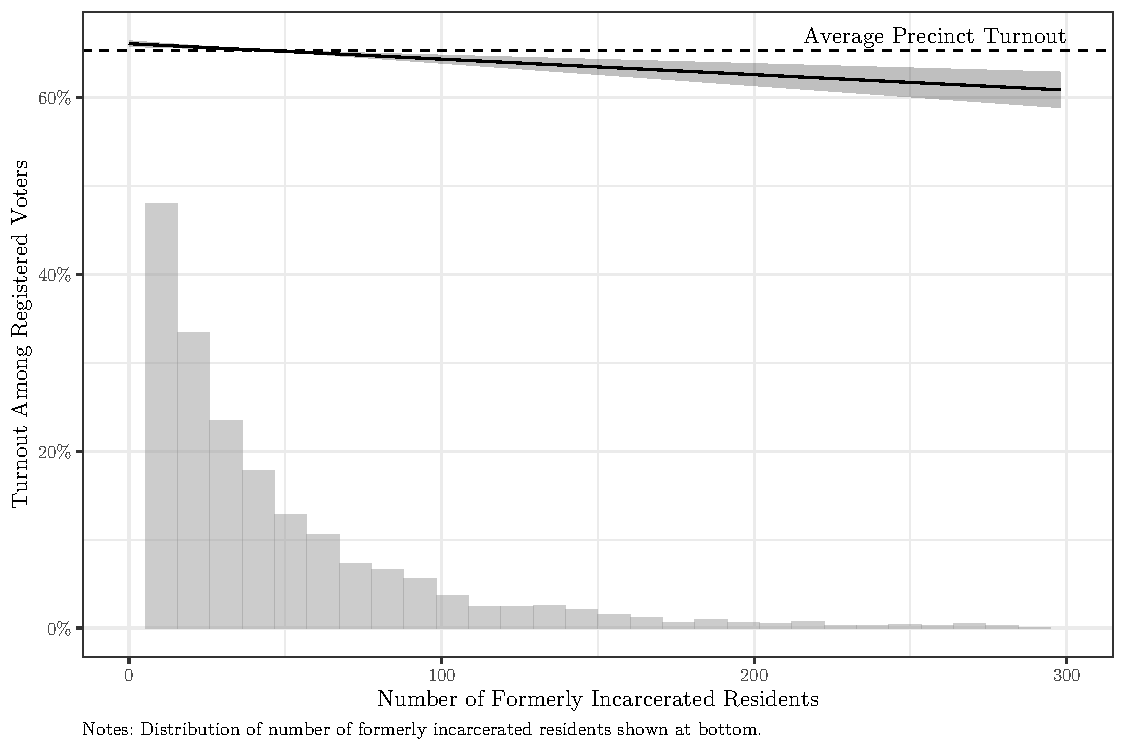
\includegraphics{amendment_4_turnout_files/figure-latex/marg1-1} 

}

\caption{\label{fig:marg1}Marginal Effect of Each Formerly Incarcerated Residents on Precinct Turnout Among Registered Voters}\label{fig:marg1}
\end{figure}

The precinct-level data allows me to test for other relationships between the number of formerly incarcerated residents in a neighborhood and that neighborhood's engagement with Amendment 4. In Table \ref{tab:other-precincts} I present the results of OLS models that test whether the number of formerly incarcerated community members influences a neighborhood's support for Amendment 4 or Amendment 4 roll-off. Roll-off is calculated as \(1 - \frac{Ballots\:Cast\:for\:Amendment\:4}{Ballots\:Cast\:in\:Contest\:with\:the\:Most\:Votes}\). It ranges from zero (if everyone who cast a ballot made a decision on the Amendment 4 question) to one (if no participants voted for or against Amendment 4). A lower number, therefore, represents lower roll-off and higher engagement.

\begin{singlespace}

\input{"../temp/precinct_other.tex"}
\end{singlespace}

Table \ref{tab:other-precincts} demonstrates that, although Amendment 4 did not boost precinct-level turnout, precincts with more formerly incarcerated residents \emph{did} support Amendment 4 at slightly higher rates. So too did precincts with fewer men and fewer registered Republicans, and where more residents had some collegiate education. Similarly, roll-off was lower in neighborhoods with formerly incarcerated residents, which means that a higher share of residents expressed a preference on the question. Thus it appears that while the presence of formerly incarcerated individuals in a neighborhood was not associated with getting people into the voting booth, it was associated with how voters cast their ballots once there. Figures \ref{fig:marg-alt} and \ref{fig:marg-alt2} plot the marginal effect of each additional formerly incarcerated resident on a precinct's support for Amendment 4, and the precinct's roll-off on Amendment 4. These figures make clear that the number of formerly incarcerated residents has a relatively small impact on precinct support for its passage, and a relatively large impact on precinct level roll-off on the question.

\begin{figure}[H]

{\centering 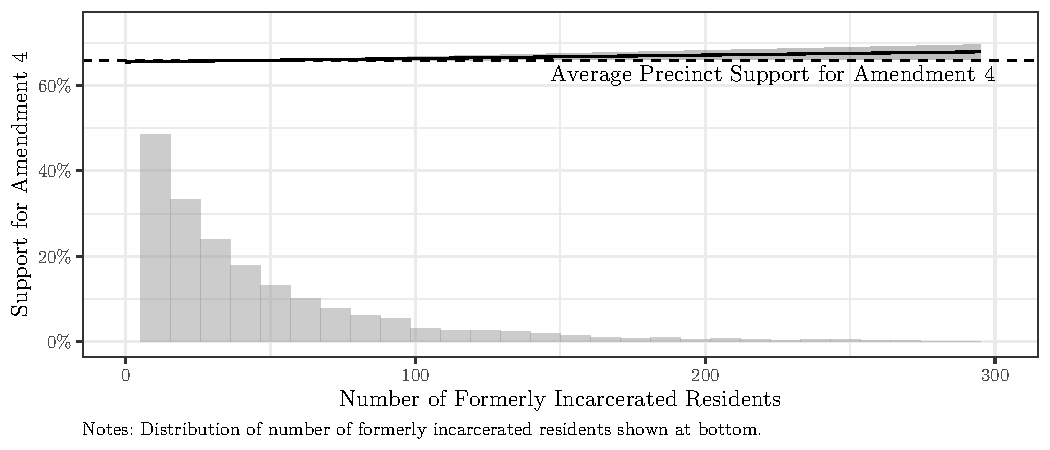
\includegraphics{amendment_4_turnout_files/figure-latex/marg-alt-1} 

}

\caption{\label{fig:marg-alt}Marginal Effect of Formerly Incarcerated Residents on Support for Amendment 4}\label{fig:marg-alt}
\end{figure}
\begin{figure}[H]

{\centering 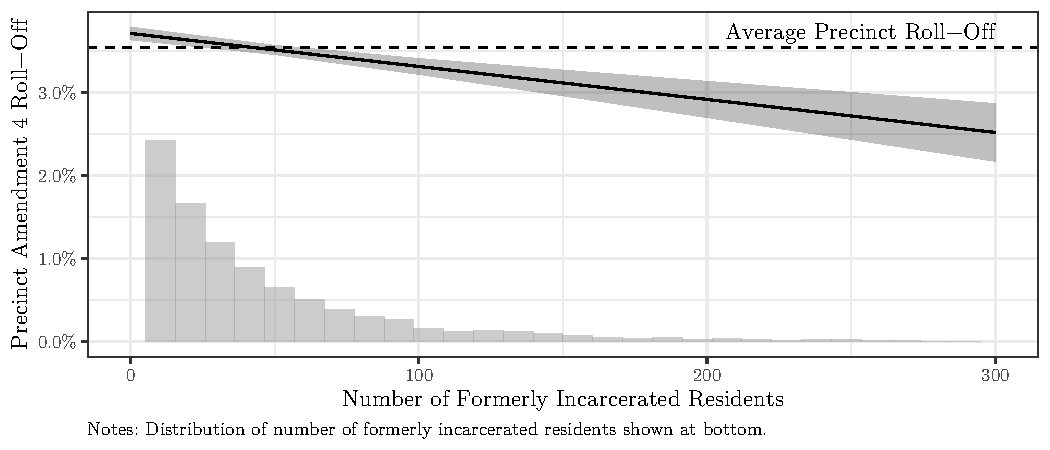
\includegraphics{amendment_4_turnout_files/figure-latex/marg-alt2-1} 

}

\caption{\label{fig:marg-alt2}Marginal Effect of Formerly Incarcerated Residents on Amendment 4 Roll-Off}\label{fig:marg-alt2}
\end{figure}

\hypertarget{individual-level-results}{%
\section*{Individual-Level Results}\label{individual-level-results}}
\addcontentsline{toc}{section}{Individual-Level Results}

Thus far I have established that neighborhoods with more formerly incarcerated residents turned out at lower rates than other neighborhoods. Although this is in line with past scholarship that has found negative indirect turnout effects from incarceration and felony disenfranchisement, it is sobering to note that even a ballot initiative that would increase these neighborhoods' political representation via the expansion of the franchise was not enough to overcome these negative effects.

The use of neighborhood data, however, can obscure underlying patterns. Encouragements to vote at the household level might be too small to register at the neighborhood level. Examining the relationship between cohabitation with formerly incarcerated individuals and turnout can shed light on the ways in which proximal contact depress turnout. It is possible that Amendment 4 shaped turnout differently for individuals who cohabitate with formerly incarcerated individuals than for their neighbors. A neighborhood may have disengaged from the political process thanks to a history of aggressive state action. Household members of the formerly incarcerated may have had a similar historical response, and yet be more susceptible to mobilization from Amendment 4's placement on the ballot; their family members and housemates, after all, are the individuals who stood to benefit from the passage of the amendment. These formerly incarcerated individuals may have successfully mobilized other members of their households but failed to do so for their neighborhood.

Using individual-level data, I here distinguish the effect of proximal neighborhood contact from individual-level contact on turnout in 2018. As discussed above, I identify individuals who live with formerly incarcerated individuals by matching addresses listed in the Department of Corrections release data to the registered voter file. All registered voters who live at an address reported by a formerly incarcerated individual are considered ``treated'' with proximal contact to the carceral state.

Each treated individual is then matched with five untreated registered voters elsewhere in her congressional district.\footnote{Due to computing constraints, a random 5 percent random sample stratified by treatment status is used to calculate the genetic weights. The full sample is used for matching.} Exact matching is done on all characteristics with the exception of registration date, age, median income, and share with some collegiate education, and matching is done with replacement. Ties are not broken, which means that some treated voters have more than five controls; the regression weights are calculated to allow for this possibility. Voters are matched using their block group's median income and share with some collegiate education (from the ACS 5 year estimates ending in 2018), while all other characteristics come from the individual-level voter file. Table \ref{tab:bal-table} presents the results of this matching exercise. In addition to the characteristics reported in Table \ref{tab:bal-table}, matches are required to come from the same congressional district to account for different levels of congressional competition in the 2018 election.

\begin{singlespace}
\begin{table}[H]

\caption{\label{tab:balance-tab-chunk}\label{tab:bal-table} Balance Table}
\centering
\resizebox{\linewidth}{!}{
\begin{tabular}[t]{lllllrrrr}
\toprule
\multicolumn{1}{c}{ } & \multicolumn{2}{c}{Means: Unmatched Data} & \multicolumn{2}{c}{Means: Matched Data} & \multicolumn{4}{c}{Percent Improvement} \\
\cmidrule(l{3pt}r{3pt}){2-3} \cmidrule(l{3pt}r{3pt}){4-5} \cmidrule(l{3pt}r{3pt}){6-9}
 & Treated & Control & Treated & Control & Mean Diff & eQQ Med & eQQ Mean & eQQ Max\\
\midrule
\%White & 42.0\% & 63.0\% & 42.0\% & 42.0\% & 100.00 & 100.00 & 100.00 & 100.00\\
\% Black & 39.0\% & 13.0\% & 39.0\% & 39.0\% & 100.00 & 100.00 & 100.00 & 100.00\\
\% Latino & 13.0\% & 17.0\% & 13.0\% & 13.0\% & 99.86 & 99.86 & 99.86 & 99.86\\
\% Asian & 1.0\% & 2.0\% & 1.0\% & 1.0\% & 100.00 & 100.00 & 100.00 & 100.00\\
\% Female & 55.0\% & 52.0\% & 55.0\% & 55.0\% & 100.00 & 100.00 & 100.00 & 100.00\\
\% Male & 42.0\% & 45.0\% & 42.0\% & 42.0\% & 99.74 & 99.74 & 99.74 & 99.74\\
Registration Date & 2004-01-28 & 2004-09-24 & 2004-01-28 & 2004-02-10 & 94.63 & 30.85 & 20.67 & 16.86\\
Age & 48.95 & 52.45 & 48.95 & 48.82 & 96.12 & 95.63 & 93.77 & 91.93\\
\% Democrat & 54.0\% & 37.0\% & 54.0\% & 54.0\% & 100.00 & 100.00 & 100.00 & 100.00\\
\% Republican & 21.0\% & 35.0\% & 21.0\% & 21.0\% & 100.00 & 100.00 & 100.00 & 100.00\\
\% with Some College & 66.0\% & 75.0\% & 66.0\% & 67.0\% & 99.88 & 99.93 & 99.89 & 99.54\\
Median Income & \$47,389 & \$62,995 & \$47,389 & \$47,401 & 99.93 & 99.85 & 99.76 & 99.32\\
\bottomrule
\end{tabular}}
\end{table}
\end{singlespace}

As Table \ref{tab:bal-table} makes clear, the treated registered voters differ in meaningful ways from the rest of the electorate: they are three times as likely to be Black, they are substantially more likely to be registered as Democrats, and they live in neighborhoods with lower incomes. The matching process, however, results in a control group that is very similar to the treatment group; in each measure, there was at least a 94 percent improvement in the mean difference.

After matching the treated voters to appropriate controls, I construct a difference-in-differences model. Before presenting the results of the model, I show in Figure \ref{fig:dind} that the parallel trends assumption is satisfied: although the treatment group has lower turnout rates in general, the distance between the treatment and control groups is largely constant between 2010 and 2016.

\begin{figure}[H]

{\centering 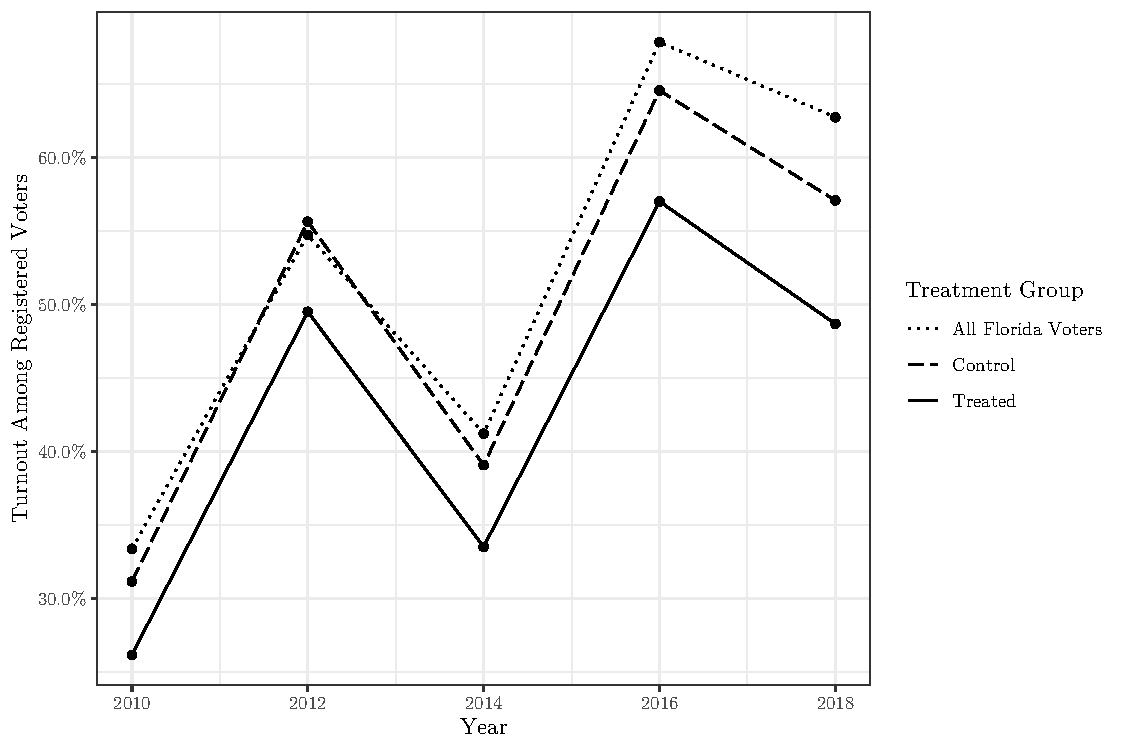
\includegraphics{amendment_4_turnout_files/figure-latex/dind-1} 

}

\caption{\label{fig:dind}General Election Turnout for Treated and Control Voters, 2010 -- 2018}\label{fig:dind}
\end{figure}

The trends presented in Figure \ref{fig:dind} offer preliminary visual corroboration of what I find at the neighborhood level --- namely, that proximal contact with formerly incarcerated individuals did not result in higher turnout in the 2018 election even after controlling for historical turnout. Table \ref{tab:tab-dind} formalizes these trends into an ordinary least-squares regression.\footnote{Although the dependent variable here is binary --- it takes the value 0 if a voter does not participate, and 1 if she does --- the coefficients produced by logistic regressions in the difference-in-differences context are largely uninterpretable. I thus use a linear specification here. When the models are estimated using a logistic specification, the treatment effect is virtually identical.} A treatment dummy distinguishes treated from control voters. The treatment dummy is interacted with another dummy identifying the 2018 election. Robust standard errors are clustered at the level of the match (Abadie and Spiess \protect\hyperlink{ref-Abadie2019}{2019}). Model 1 presents the model output without the other controls used for matching; Model 2 includes these covariates.

In Models 3 and 4 of Table \ref{tab:tab-dind} I consider the possibility that, as households become further removed from a member's incarceration, the negative effects of their incarceration on turnout dissipate. In these models, the dummies indicating treatment and the 2018 election are interacted with the number of years since the most recent completion of a term of incarceration for a household member. Matched control observations are assigned the value associated with their treated observation. Model 3 includes no other covariates, while Model 4 includes the matched variables.

It is, of course, highly possible that formerly incarcerated individuals no longer live in the same household they reported when leaving prison; this is especially true for individuals released from prison early in the sample. To control for this possibility, Models 5 -- 8 include only the treated individuals (and their matches) whose registration dates are earlier than the latest prison release date of a household member. These are individuals, therefore, that we can be sure lived with an incarcerated individual. The treatment effects in these models, though slightly larger, tell the same general story.

\begin{singlespace}
\input{"../temp/dind_reg.tex"}
\end{singlespace}

In each of the specifications presented in Table \ref{tab:tab-dind}, treated individuals were less likely to vote in 2018 after controlling for both their own vote history and the vote history of their matched counterparts. The coefficients on \emph{D(2018) × D(Treated)} in Models 1 and 2 indicate that turnout among treated voters was about 2.3 percentage points below what it would have been if 2018 had conformed to prior years.

The models that incorporate information about how long their housemates had been out of prison indicate, however, that this effect is moderated by time: individuals who lived with housemates who had not been imprisoned in many years were more likely to vote in 2018 than other treated voters. TModels 3 and 4 estimate that the treatment effect for individuals whose household member returned from prison within one year of the election was about -4.0 percentage points, but that for each year the most recent incarceration recedes into the past, the treatment effect decreases by about 0.2 percent.

That the effect is moderated by time is unsurprising. Individuals whose household members went to and were released from prison between the 2016 and 2018 elections, for instance, received two treatments: they both were ``negatively'' treated by their proximal contact with the criminal justice system and potentially ``positively'' treated by the presence of Amendment 4. What \emph{is} surprising, however, is the continued negative treatment effect even for the households that were most removed from their proximal contact with the incarceration of a household member. Table \ref{tab:oldies} presents the results of Models 5 and 6 from Table \ref{tab:tab-dind}, but limits the pool to households where the most recent incarceration ended prior to 2010. This pool is restricted to individuals we are certain lived with formerly incarcerated individuals, and the negative shock of proximal contact for these individuals should be reflected in the base years of the difference-in-differences models. That \emph{D(2018) × D(Treated)} remains significant and negative for these individuals is puzzling.

\begin{singlespace}
\input{"../temp/dind_reg_medium.tex"}
\end{singlespace}

This negative, significant finding for treated individuals whose household members had been out of prison for many years should probably not be interpreted to mean that Amendment 4 had a demobilizing effect on individuals in proximal contact to formerly incarcerated individuals. Rather, it likely points to meaningful differences in susceptibility to broad mobilization for those in proximal contact with the criminal justice system. The 2018 election was historic in many ways: according to the United States Elections Project,\footnote{\url{http://www.electproject.org/home/voter-turnout/voter-turnout-data}.} turnout was higher than it had been for a midterm election in a century. Many marginal voters who had not previously participated in midterm elections turned out. This is readily apparent in Figure \ref{fig:dind} --- the turnout in 2018 for the control and treatment groups was far higher than in 2014 or 2010. The control group, in fact, turned out at higher rates in 2018 than in the presidential contest of 2012, and the same was nearly true for the treatment group. The negative treatment effect for the treatment group in 2018 likely arises more from the unique nature of the 2018 election than from any demobilizing effect of Amendment 4.

And yet, this negative treatment effect is troubling. As Table \ref{tab:bal-table} indicates, the matching procedure was successful at creating a control group that looks nearly identical to the treatment group --- \emph{according to observable characteristics}. Not only did Amendment 4 fail to mobilize voters who live in close proximity to the formerly incarcerated; it appears that these voters are also \emph{less} mobilized by the same factors that encourage similar voters to participate in unique elections such as that of 2018. This analysis cannot determine whether the proximal contact caused this imperviousness to broadly mobilizing conditions, or if individuals who live in close proximity to the formerly incarcerated would have been more likely to remain on the sidelines in an election like 2018 even without the proximal contact in their past. Nevertheless, their relatively depressed turnout in 2018 --- even in the presence of Amendment 4 on the ballot --- underscores just how difficult their political (re)integration is.

\hypertarget{discussion-and-conclusion}{%
\section*{Discussion and Conclusion}\label{discussion-and-conclusion}}
\addcontentsline{toc}{section}{Discussion and Conclusion}

Turnout in 2018 hit historic levels for a midterm election as infrequent voters participated and made their voices heard. In addition to hotly contested Congressional, senate, and gubernatorial races, Floridians were presented with the opportunity to restore voting rights to well over a million permanently disenfranchised individuals who had been convicted of felony offenses. Amendment 4 and its organizers were hugely successful --- in a year where both statewide winners won by less than 0.5 percentage points, nearly two-thirds of Flordians supported expanding the franchise. Neighborhoods and voters most directly impacted by felony disenfranchisement stood to gain meaningful political representation from the passage of the amendment. Despite ongoing litigation (Stern \protect\hyperlink{ref-Stern2020}{2020}), the amendment is poised to do just that.

And these proximal voters \emph{did} turn out at higher rates in 2018 than in previous elections: as Figure \ref{fig:dind} demonstrates, turnout among voters who live with formerly incarcerated individuals increased by more than 15 percentage points --- or 45 percent --- between 2014 and 2018. And their neighborhoods overwhelmingly supported the passage of the amendment; moreover, the presence of formerly incarercated individuals measurably increased the degree to which a neighborhood supported and engaged with the amendment.

Despite these major gains in turnout among individuals in proximate contact with the carceral state, I fail to uncover evidence that the presence of Amendment 4 increased the turnout among these individuals above-and-beyond the increases observed among other voters and in other communities. Although these residents of directly impacted communities stood to benefit disproportionately from the passage of Amendment 4, they were not more likely to participate than similarly situated voters without that proximal contact. In fact, the evidence points in the opposite direction: turnout for these voters actually increased \emph{less} in 2018 than it did for other voters. Not only was Amendment 4 not particularly mobilizing, but these voters are also less susceptible to factors contributing to statewide surges in turnout. Once these voters were in the voting booth, however, they were less likely to roll-off and more likely to vote yes on Amendment 4.

Why the voters who were likely to benefit the most were not more likely to vote is not immediately apparent. It could be an issue of voter knowledge; previous research has indicated that marginalized voters demonstrate lower political knowledge (Erikson \protect\hyperlink{ref-Erikson2015}{2015}). If these proximal contact voters were not aware that Amendment 4 was on the ballot, the amendment could hardly have mobilized them to vote. This could be especially true in ballot initiatives where resources are tight: campaigns such as the Florida Rights Restoration Coalition may have focused on contacting higher income, higher propensity voters, even though these voters were less likely to directly benefit from the passage of the amendment. Further research is needed to understand how and why these communities were not more likely to vote than their counterparts.

Whatever the causal mechanism that resulted in lower turnout for these communities despite the presence of Amendment 4, the results point to the next chapter of the fight for political integration and representation for advocates in the Sunshine State. The relatively lower turnout in 2018 for the communities most impacted by the carceral state indicates that formal re-enfranchisement is not enough; if Floridian and American democracy wants to \emph{actually} incorporate voices from these communities --- and not simply legally \emph{allow} for their incorporation --- the advocacy movement cannot consider its work done once the formal barriers to the ballot box have been torn down. Re-enfranchisement is clearly necessary, but it is not sufficient. Researchers must continue exploring why the political re-incorporation of these communities is so difficult, and advocates on the ground must do the hard work of reknitting them to our body politic.

\newpage

\hypertarget{supplementary-information}{%
\section*{Supplementary Information}\label{supplementary-information}}
\addcontentsline{toc}{section}{Supplementary Information}

When discussing the impact of formerly incarcerated residents on neighborhood turnout and support for Amendment 4 in the body of this paper, I include only a subset of formerly incarcerated residents. I exclude individuals who returned from prison to institutions listed by four or more other formerly incarcerated individuals. I choose to exclude these individuals because I am most interested in the relationship between Amendment 4 and the turnout of individuals in proximal contact with the criminal justice system. Walker and García-Castañon (\protect\hyperlink{ref-Walker2017}{2017}) defines proximal contact ``as having a loved one who is a custodial citizen without yourself having had contact'' (542). Because much of the literature focuses on the mechanisms linking personal relationships, proximal contact, and political participation, I limit the sample to formerly incarcerated individuals who are likely returning to neighborhoods with social and familial ties.

Nevertheless, individuals who live in neighborhoods with large numbers of formerly incarcerated individuals who reside in institutions like half-way houses or shelters do have a different sort of proximal contact with the criminal justice system: many of the neighbors they interact with have been to prison, but these individuals do not necessarily have strong filial or social relationships with other residents. I begin this appendix by re-estimating the models presented in Tables \ref{tab:to-precinct} and \ref{tab:other-precincts} in the body of this paper, but now including \emph{all} formerly incarcerated residents. Table \ref{tab:ap-a-1} presents the results of these estimations. Model 1 presents the turnout regression estimated at the block group level, while Models 2 -- 4 are estimated using precinct level data.

\begin{singlespace}

\input{"../temp/ap_a_1.tex"}
\end{singlespace}

The inclusion of all formerly incarcerated residents substantially shrinks the size of the estimated coefficients of interest with respect to the estimates presented in the body of the paper. Nevertheless, turnout (measured at the block group and precinct level) and roll-off are significantly and negatively related with the formerly incarcerated population in a neighborhood, and support for Amendment 4 remains positively (and significantly) related. It appears, then, that formerly incarcerated residents who return to institutions have smaller spillover effects on their neighbors' voting behavior.

The body of the paper also acknowledges that the use of release-address data may be unreliable considering the fact that many individuals may have moved or died since their discharge from parole. This is especially possible for individuals who have not had contact with the state incarceration agency for many years. To account for this possibility, Table \ref{tab:ap-a-2} re-estimates the models presented in Tables \ref{tab:to-precinct} and \ref{tab:other-precincts}, but limits the formerly incarcerated individuals to those residents who were last discharged from parole between 2015 and the 2018 election. These individuals are the least likely to have died or moved, simply because their information is the most recent. These models include only individuals who returned to non-institutions, as presented in the body of the paper.

\begin{singlespace}

\input{"../temp/ap_a_2.tex"}
\end{singlespace}

In each of the models presented in Table \ref{tab:ap-a-2}, the independent variable of interest is statistically significant at the 99 percent level. Moreover, the estimated coefficient is in each case larger than that presented in the body of the paper. This could be because using more recent data better identifies communities that are currently home, not just historically home, to formerly incarcerated individuals. On the other hand, a community member's incarceration may be more salient in places where residents were more recently incarcerated. Proximal contact, in other words, might shape voters' behavior more strongly if that contact was recent. The individual-level difference-in-differences regressions presented later in the paper would seem to corroborate this as well.

\newpage

\hypertarget{references}{%
\section*{References}\label{references}}
\addcontentsline{toc}{section}{References}

\hypertarget{refs}{}
\begin{cslreferences}
\leavevmode\hypertarget{ref-Abadie2019}{}%
Abadie, Alberto, and Jann Spiess. 2019. ``Robust Post-Matching Inference.'' \emph{Working Paper.}

\leavevmode\hypertarget{ref-Amos2020}{}%
Amos, Brian, and Michael P. McDonald. 2020. ``A Method to Audit the Assignment of Registered Voters to Districts and Precincts.'' \emph{Political Analysis}, 1--16. \url{https://doi.org/10.1017/pan.2019.44}.

\leavevmode\hypertarget{ref-Amos2017}{}%
Amos, Brian, Michael P. McDonald, and Russell Watkins. 2017. ``When Boundaries CollideConstructing a National Database of Demographic and Voting Statistics.'' \emph{Public Opinion Quarterly} 81 (S1): 385--400. \url{https://doi.org/10.1093/poq/nfx001}.

\leavevmode\hypertarget{ref-Austin2004}{}%
Austin, Regina. 2004--2005. ``The Shame of It All: Stigma and the Political Disenfranchisement of Formerly Convicted and Incarcerated Persons Symposium on Race, Crime, and Voting: Social, Political, and Philosophical Perspectives on Felony Disenfranchisement in America.'' \emph{Columbia Human Rights Law Review} 36 (1): 173--92. \url{https://heinonline.org/HOL/P?h=hein.journals/colhr36\&i=181}.

\leavevmode\hypertarget{ref-Baumann2019}{}%
Baumann, Joella. 2019. ``Paroled Coloradans Are Now Eligible to Vote.'' \emph{Colorado Public Radio}, July 1, 2019. \url{https://www.cpr.org/2019/07/01/paroled-coloradans-are-now-eligible-to-vote/}.

\leavevmode\hypertarget{ref-Berman2018}{}%
Berman, Ari. 2018. ``Inside the Unlikely Movement That Could Restore Voting Rights to 1.4 Million Floridians.'' \emph{Mother Jones: Politics}, November 2018. \url{https://www.motherjones.com/politics/2018/10/inside-the-unlikely-movement-that-could-restore-voting-rights-to-1-4-million-floridians/}.

\leavevmode\hypertarget{ref-Bowers2009}{}%
Bowers, Melanie, and Robert R. Preuhs. 2009. ``Collateral Consequences of a Collateral Penalty: The Negative Effect of Felon Disenfranchisement Laws on the Political Participation of Nonfelons*.'' \emph{Social Science Quarterly} 90 (3): 722--43. \url{https://doi.org/10.1111/j.1540-6237.2009.00640.x}.

\leavevmode\hypertarget{ref-Burch2011}{}%
Burch, Traci. 2011. ``Turnout and Party Registration Among Criminal Offenders in the 2008 General Election.'' \emph{Law \& Society Review} 45 (3): 699--730. \url{https://doi.org/10.1111/j.1540-5893.2011.00448.x}.

\leavevmode\hypertarget{ref-Burch2013}{}%
Burch, Traci R. 2013. ``Effects of Imprisonment and Community Supervision on Neighborhood Political Participation in North Carolina:'' \emph{The ANNALS of the American Academy of Political and Social Science}, November. \url{https://doi.org/10.1177/0002716213503093}.

\leavevmode\hypertarget{ref-Bushway2007}{}%
Bushway, Shawn D., Michael A. Stoll, and David Weiman. 2007. \emph{Barriers to Reentry?: The Labor Market for Released Prisoners in Post-Industrial America}. Russell Sage Foundation. \url{http://books.google.com?id=YOeFAwAAQBAJ}.

\leavevmode\hypertarget{ref-Crisp2019}{}%
Crisp, Elizabeth. 2019. ``Thousands of Felons in Louisiana Will Regain Voting Rights When This Law Takes Effect March 1.'' \emph{The Advocate}, February 15, 2019. \url{https://www.theadvocate.com/baton_rouge/news/politics/article_8a73810c-3153-11e9-81bd-97a9537e8c8b.html}.

\leavevmode\hypertarget{ref-Erikson2015}{}%
Erikson, Robert S. 2015. ``Income Inequality and Policy Responsiveness.'' \emph{Annual Review of Political Science} 18 (1): 11--29. \url{https://doi.org/10.1146/annurev-polisci-020614-094706}.

\leavevmode\hypertarget{ref-bcj_laws}{}%
Justice, Brennan Center for. 2019. ``Criminal Disenfranchisement Laws Across the United States.'' \emph{Brennan Center for Justice}, May. \url{https://www.brennancenter.org/our-work/research-reports/criminal-disenfranchisement-laws-across-united-states}.

\leavevmode\hypertarget{ref-Kelso2018}{}%
Kelso, Nathaniel, and Michael Migurski. 2018. ``Election-Geodata.'' 2018. \url{https://github.com/nvkelso/election-geodata}.

\leavevmode\hypertarget{ref-King2016}{}%
King, Bridgett A., and Laura Erickson. 2016. ``Disenfranchising the Enfranchised: Exploring the Relationship Between Felony Disenfranchisement and African American Voter Turnout.'' \emph{Journal of Black Studies}, July. \url{https://doi.org/10.1177/0021934716659195}.

\leavevmode\hypertarget{ref-Knack2008}{}%
Knack, Stephen, and Martha Kropf. 2008. ``Roll-Off at the Top of the Ballot: International Undervoting in American Presidential Elections.'' \emph{Politics \& Policy} 31 (4): 575--94. \url{https://doi.org/10.1111/j.1747-1346.2003.tb00163.x}.

\leavevmode\hypertarget{ref-Lerman2014}{}%
Lerman, Amy E., and Vesla M. Weaver. 2014. \emph{Arresting Citizenship: The Democratic Consequences of American Crime Control}. Chicago Studies in American Politics. Chicago ; London: The University of Chicago Press.

\leavevmode\hypertarget{ref-Martin2018}{}%
Martin, Karin D., Bryan L. Sykes, Sarah Shannon, Frank Edwards, and Alexes Harris. 2018. ``Monetary Sanctions: Legal Financial Obligations in US Systems of Justice.'' \emph{Annual Review of Criminology} 1 (1): 471--95. \url{https://doi.org/10.1146/annurev-criminol-032317-091915}.

\leavevmode\hypertarget{ref-Mcdonald2002}{}%
Mcdonald, Michael P. 2002. ``The Turnout Rate Among Eligible Voters in the States, 1980--2000.'' \emph{State Politics \& Policy Quarterly} 2 (2): 199--212. \url{https://doi.org/10.1177/153244000200200205}.

\leavevmode\hypertarget{ref-Mettler2002}{}%
Mettler, Suzanne. 2002. ``Bringing the State Back in to Civic Engagement: Policy Feedback Effects of the G.I. Bill for World War II Veterans.'' \emph{The American Political Science Review} 96 (2): 351--65. \url{http://www.jstor.org/stable/3118030}.

\leavevmode\hypertarget{ref-Mettler2004}{}%
Mettler, Suzanne, and Joe Soss. 2004. ``The Consequences of Public Policy for Democratic Citizenship: Bridging Policy Studies and Mass Politics.'' \emph{Perspectives on Politics} 2 (1): 55--73. \url{http://www.jstor.org/stable/3688340}.

\leavevmode\hypertarget{ref-Miles2004}{}%
Miles, Thomas J. 2004. ``Felon Disenfranchisement and Voter Turnout.'' \emph{The Journal of Legal Studies} 33 (1): 85--129. \url{https://doi.org/10.1086/381290}.

\leavevmode\hypertarget{ref-Morris2018}{}%
Morris, Kevin. 2018. ``A Transformative Step for Democracy in Florida.'' Brennan Center for Justice. November 7, 2018. \url{https://www.brennancenter.org/our-work/analysis-opinion/transformative-step-democracy-florida}.

\leavevmode\hypertarget{ref-Morris2020}{}%
---------. 2020. ``Neighborhoods and Felony Disenfranchisement: The Case of New York City.'' \emph{Urban Affairs Review}, May, 1078087420921522. \url{https://doi.org/10.1177/1078087420921522}.

\leavevmode\hypertarget{ref-Naser2006}{}%
Naser, Rebecca L, and Christy A Visher. 2006. ``Family Members' Experiences with Incarceration and Reentry,'' 12.

\leavevmode\hypertarget{ref-Robles2018}{}%
Robles, Frances. 2018. ``1.4 Million Floridians with Felonies Win Long-Denied Right to Vote.'' \emph{The New York Times: U.S.}, November 7, 2018. \url{https://www.nytimes.com/2018/11/07/us/florida-felon-voting-rights.html}.

\leavevmode\hypertarget{ref-Sekhon2011}{}%
Sekhon, Jasjeet S. 2011. ``Multivariate and Propensity Score Matching Software with Automated Balance Optimization: The Matching Package for R.'' \emph{Journal of Statistical Software} 42 (1): 1--52. \url{https://doi.org/10.18637/jss.v042.i07}.

\leavevmode\hypertarget{ref-Smith2018}{}%
Smith, Jamil, and Jamil Smith. 2018. ``Andrew Gillum Is Ready. Is Florida?'' Rolling Stone. October 31, 2018. \url{https://www.rollingstone.com/politics/politics-features/andrew-gillum-florida-governor-race-749651/}.

\leavevmode\hypertarget{ref-Stern2019}{}%
Stern, Mark Joseph. 2019. ``Florida Republicans Are Sabotaging a Constitutional Amendment That Gave Felons the Right to Vote.'' Slate Magazine. March 20, 2019. \url{https://slate.com/news-and-politics/2019/03/florida-republicans-felon-voting-rights-amendment-4.html}.

\leavevmode\hypertarget{ref-Stern2020}{}%
---------. 2020. ``Florida Can't Bar Ex-Felons from Voting Just Because They're Poor, Appeals Court Rules.'' Slate Magazine. February 19, 2020. \url{https://slate.com/news-and-politics/2020/02/amendment-4-eleventh-circuit-florida-voting.html}.

\leavevmode\hypertarget{ref-Taylor2018}{}%
Taylor, Adam. 2018. ``Florida's Move to Allow Ex-Felons to Vote Brings U.S. Closer to International Election Norms.'' \emph{Washington Post: WorldViews}, November 7, 2018. \url{https://www.washingtonpost.com/world/2018/11/07/floridas-move-allow-ex-felons-vote-brings-us-closer-international-election-norms/}.

\leavevmode\hypertarget{ref-sentencing_2016}{}%
Uggen, Christopher, Ryan Larson, and Sarah Shannon. 2016. ``6 Million Lost Voters: State-Level Estimates of Felony Disenfranchisement, 2016.'' Research report. The Sentencing Project. \url{https://www.sentencingproject.org/publications/6-million-lost-voters-state-level-estimates-felony-disenfranchisement-2016/}.

\leavevmode\hypertarget{ref-USPS2015}{}%
USPS. 2015. ``Appendix C.'' Postal Addressing Standards. May 2015. \url{https://pe.usps.com/text/pub28/28apc_002.htm}.

\leavevmode\hypertarget{ref-Vanderleeuw1987}{}%
Vanderleeuw, James M., and Richard L. Engstrom. 1987. ``Race, Referendums, and Roll-Off.'' \emph{The Journal of Politics} 49 (4): 1081--92. \url{https://doi.org/10.2307/2130785}.

\leavevmode\hypertarget{ref-bcj_iowa}{}%
``Voting Rights Restoration Efforts in Iowa.'' 2020. Brennan Center for Justice. 2020. \url{https://www.brennancenter.org/our-work/research-reports/voting-rights-restoration-efforts-iowa}.

\leavevmode\hypertarget{ref-Walker2014}{}%
Walker, Hannah L. 2014. ``Extending the Effects of the Carceral State: Proximal Contact, Political Participation, and Race.'' \emph{Political Research Quarterly}, July. \url{https://doi.org/10.1177/1065912914542522}.

\leavevmode\hypertarget{ref-Walker2020}{}%
---------. 2020. ``Targeted: The Mobilizing Effect of Perceptions of Unfair Policing Practices.'' \emph{The Journal of Politics} 82 (1): 119--34. \url{https://doi.org/10.1086/705684}.

\leavevmode\hypertarget{ref-Walker2017}{}%
Walker, Hannah L., and Marcela García-Castañon. 2017. ``For Love and Justice: The Mobilizing of Race, Gender, and Criminal Justice Contact.'' \emph{Politics \& Gender} 13 (4): 541--68. \url{https://doi.org/10.1017/S1743923X17000198}.

\leavevmode\hypertarget{ref-Wang2018}{}%
Wang, Vivian. 2018. ``Cuomo Plans to Restore Voting Rights to Paroled Felons.'' \emph{The New York Times: New York}, April 18, 2018. \url{https://www.nytimes.com/2018/04/18/nyregion/felons-pardon-voting-rights-cuomo.html}.

\leavevmode\hypertarget{ref-Wattenberg2000}{}%
Wattenberg, Martin P., Ian McAllister, and Anthony Salvanto. 2000. ``How Voting Is Like Taking an Sat Test: An Analysis of American Voter Rolloff.'' \emph{American Politics Quarterly} 28 (2): 234--50. \url{https://doi.org/10.1177/1532673X00028002005}.

\leavevmode\hypertarget{ref-Weaver2010}{}%
Weaver, Vesla M., and Amy E. Lerman. 2010. ``Political Consequences of the Carceral State.'' \emph{American Political Science Review} 104 (4): 817--33. \url{https://doi.org/10.1017/S0003055410000456}.

\leavevmode\hypertarget{ref-White2019a}{}%
White, Ariel. 2019a. ``Family Matters? Voting Behavior in Households with Criminal Justice Contact.'' \emph{American Political Science Review} 113 (2): 607--13. \url{https://doi.org/10.1017/S0003055418000862}.

\leavevmode\hypertarget{ref-White2019}{}%
---------. 2019b. ``Misdemeanor Disenfranchisement? The Demobilizing Effects of Brief Jail Spells on Potential Voters.'' \emph{American Political Science Review} 113 (2): 311--24. \url{https://doi.org/10.1017/S000305541800093X}.

\leavevmode\hypertarget{ref-Wines2019}{}%
Wines, Michael. 2019. ``Kentucky Gives Voting Rights to Some 140,000 Former Felons.'' \emph{The New York Times: U.S.}, December 12, 2019. \url{https://www.nytimes.com/2019/12/12/us/kentucky-felons-voting-rights.html}.
\end{cslreferences}

\end{document}
